Studiamo adesso in dettaglio il legame chimico.

Ciò significa che studieremo il legame nelle molecole, sebbene sappiamo che ci sono molti sistemi che non esistono sotto forma molecolare ossia i composti ionici, dei quali conosciamo i solidi ma non le molecole. Ne è un esempio l'NaCl: la specie molecolare del cloruro di sodio non esiste, ma esiste il solido.

Dobbiamo allora comprendere perché non esistano le molecole singole delle speci fortementi ioniche, per poi ragionare sul legame chimico, che ha una natura diversa nei sistemi molecolari.

Dobbiamo quindi rispondere a una serie di domande:
\begin{itemize}
    \item Perché si formano le molecole, dato che molti sistemi non esistono come tali?
    \item Quali condizioni bisogna soddisfare affinché il composto che si forma a seguito di una reazione, sia stabile?
    \item Perché esistono geometrie ben definite?
\end{itemize}
Prima di andare avanti va da ricordare che in linea generale se facciamo reagire una specie A con una specie B otterremo una specie C in modo spontaneo solo se l'energia del sistema diminuisce. 

Ricordiamo poi che qualunque stato legato avrà un'energia potenziale negativa: in un sistema AB dove A e B sono due atomi, essi sono legati se la loro energia potenziale è minore di zero. Se per qualche motivo l'energia dovesse aumentare, nell'istante in cui essa diventasse pari a zero gli atomi non sarebbero più legati.

Ragioniamo solo sull'energia potenziale per via dell'esistenza del teorema del viriale, il quale afferma che

"\textit{La variazione dell'energia totale di un sistema ha lo stesso segno della variazione dell'energia potenziale}"

Quindi la molecola AB si formerà nel momento in cui l'energia potenziale dei due atomi A e B diminuisce (fino a diventare negativa) man mano che li avviciniamo.\\

Per una molecola o un sistema di pochi atomi siamo in grado di fare ragionamenti estremamente sofisticati anche se non riusciamo a risolvere con esattezza l'equazione di Schrödinger ma solo in maniera ragionevolmente approssimata, nel senso che le soluzioni ottenute non si discotano molto da valori che si ottengono sperimentalmente, ossia la descrizione approssimata risulta essere estremamente accurata per le capacità di calcolo e di modellizzazione ad oggi a disposizione.

Per essi si usa la teoria degli orbitali molecolari, che vedremo dopo.

Nell'istante in cui invece i sistemi che indaghiamo diventano complessi (molti atomi, molecole grandi con elevati pesi molecolari), non siamo più in grado, solo per esigenze di calcolo, di ottenere soluzioni approssimate ragionevolmente

Per essi allora bisogna usare una catalogazione precedente, che si basava sul tipo di legame presente tra le molecole in esame.
Un parametro estremamente utile a comprendere i sistemi è il concetto di elettronegatività, che è la tendenza che hanno i diversi atomi ad attrarre su di sé la carica di legame. Nel momento in cui uno dei due atomi costituenti il nucleo è abbastanza più elettronegativo dell'altro, si avrà una dislocazione della carica di legame, per cui diremo che la molecola avrà una sua polarità, ossia avrà struttura simile a quella di un dipolo perché avrà una parziale carica positiva e una parziale carica negativa.

In base al valore della differenza di elettronegatività, il legame verrà etichettato in vari modi:
\begin{itemize}
    \item Se è piccola (fino a 0.4) si parla di \textbf{legame covalente};
    \item Se inizia a crescere ma è comunque contenuta (da 0.4 fino a 1.9) si parla di \textbf{legame} covalente \textbf{polare}, e la molecola avrà una polarità cospicua. 
    \item Se diventa molto grande (da 1.9 in poi) si parla di \textbf{legame ionico}.
\end{itemize} 
\subsection{Il legame polare}
In questo caso ci saranno parziali cariche positive e negative, che possono venire indicate in diversi modi: o rispettivamente con $\delta^+$ e $\delta^-$, o con zone rosse e blu che indicano rispettivamente addensamento di elettroni e le zone che si sono positivizzate, o con una freccia con la punta e una croce, dove la punta è rivolta verso l'atomo più elettronegativo.
%In chimica, la polarità è una proprietà delle molecole per cui una molecola (detta polare) presenta una carica parziale positiva su una parte della molecola e una carica parziale negativa sulla parte opposta di essa. Le molecole che non presentano il fenomeno della polarità sono dette apolari o non polari.
\subsection{Il legame metallico}
Per i sistemi metallici è possibile immaginare che gli elettroni siano abbastanza liberi, tanto da essere considerati come un gas che statisticamente neutralizza i nuclei

\begin{figure}[htp]
    \centering
    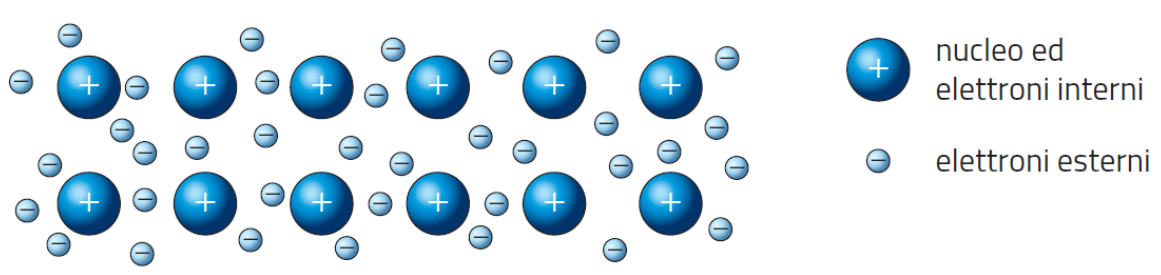
\includegraphics[width=12cm]{immagini/legame-metallico.png}
\end{figure}

Nei metalli gli atomi occupano posizioni ben definite all'interno di una struttura cristallina. A differenza dei composti ionici però qua non possiamo parlare di ioni: gli atomi sono neutri, solo che i loro elettroni esterni occupano una banda e non più un livello.

\subsection{Esempi vari}
$\bullet$ ES1 \ce{F_2}

\begin{figure}[htp]
    \centering
    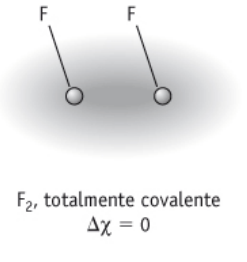
\includegraphics[width=4cm]{immagini/F_2.png}
\end{figure}

Due atomi di fluoro formano la molecola F$_2$. Sebbene il fluoro sia estremamente negativo, i due atomi sono uguali, per cui la differenza in elettronegatività è pari a zero, quindi la condivisione dei due elettroni di legame è totale e il sistema è covalente.

$\bullet$ ES2 HF

\begin{figure}[htp]
    \centering
    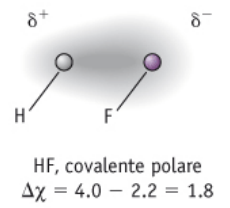
\includegraphics[width=5cm]{immagini/HF.png}
\end{figure}
Nell'acido fluoridrico la differenza di elettronegatività tra i due atomi è cospicua, e infatti la carica di legame(che può essere immaginata come una nube elettronica che circonda i due atomi) sarà più spostata verso l'atomo di fluoro e quindi meno presente sull'idrogeno. Il legame sarà allora covalente polare, con una parziale carica negativa $\delta^-$ sul fluoro e una parziale carica positiva $\delta^+$ sull'idrogeno. 

$\bullet$ ES3 LiF

\begin{figure}[htp]
    \centering
    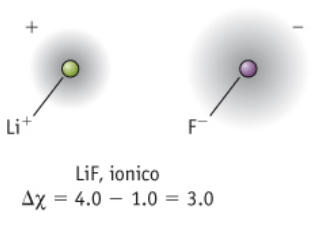
\includegraphics[width=5cm]{immagini/LiF.png}
\end{figure}

In un sistema come il fluoruro di litio, la differenza di elettronegatività è elevata, per cui non ci sarà la nube continua tra i due atomi.

Per questi sistemi si immagina che si abbia una cessione di elettroni, per cui non avremo Li e F ma Li$^+$ e F$^-$, cioè è come se il litio avesse ceduto il suo elettrone di valenza al fluoro, il quale tralaltro acquistandolo avrà la configurazione elettronica esterna dei gas nobili.
Un sistema siffatto è etichettato sistema ionico.

$\bullet$ ES4

\begin{figure}[htp]
    \centering
    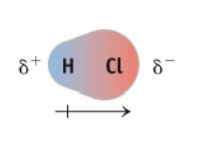
\includegraphics[width=5cm]{immagini/HCl.png}
\end{figure}

Nell'acido cloridrico la differenza di elettronegatività tra idrogeno e cloro è abbastanza evidente, per cui il legame è covalente polare.

Dato che stiamo ipotizzando che su tale molecola ci sia una buona polarità, come conseguenza ci aspettiamo un momento di dipolo.
Per verificarne l'esistenza basta mettere dell'HCl gassoso in un contenitore dove presenti le espansioni polari di un elettromagnete. Se il campo elettrico è nullo, l'orientazione delle molecole sarà casuale; se invece applichiamo una differenza di potenziale tra le due piastre osserveremo che le molecole si orientano in modo tale che il cloro sia rivolto verso la lamina positiva (a potenziale maggiore). Come facciamo ad accorgercene?
Il sistema che si viene così a costituire è un condensatore, dove tra le armature anziché il vuoto c'è un dielettrico: l'HCl. In questo modo possiamo quindi misurare il momento di dipolo, la cui unitòìà di misura nel SI è il Coulomb per metro, con cui le molecole danno dei valori dell'ordine di 10$^{-30}$, per cui si una un'altra unità di misura che è il Debye (D). Vale la relazione:
$$1D=3.336\cdot10^{-30}$$
Per l'acido cloridrico si misura un momento di dipolo pari a 1.03 D.

$\bullet$ ES5 \ce{CO_2}

\begin{figure}[htp]
    \centering
    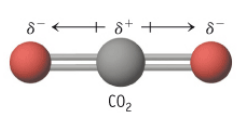
\includegraphics[width=5cm]{immagini/CO_2.png}
\end{figure}

Descrivendo l'anidride carbonica col formalismo di Lewis notavamo che sul carbonio non ci sono coppie solitarie, perché raggiunge l'ottetto grazie ai due doppi legami carbonio-ossigeno, mentre su ciascun ossigeno ce ne sono due. La geometria che tiene più lontani gli i due atommi di ossigeno con le coppie di elettroni rimaste è quella lineare.
La differenza in elettronegatività tra carbonio e ossigeno è cospicua, quindi singolarmente troviamo un momento di dipolo nei due diversi legami, ma questi si annullano a vicenda perché sono uguali in modulo ma opposti in verso. Pertanto questa molecola ha un momento di dipolo netto pari a zero, cioè non è polare, pur essendo polari i singoli legami.

$\bullet$ ES6 \ce{H_2O}

\begin{figure}[htp]
    \centering
    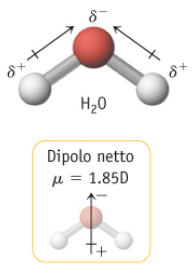
\includegraphics[width=5cm]{immagini/H_2O.png}
\end{figure}

Descrivendo l'acqua col formalismo di Lewis notavamo due coppie solitarie sull'ossigeno. Dovendo ragionare su un sistema con 4 coppie di elettroni usiamo l'idea del sistema tetraedrico nel quale però le due coppie solitarie stringono il legame, che avrà un angolo di 104.5°. Considerando solo gli atomi, questa molecola sarà piana ma angolata.

La differenza in elettronegatività tra idrogeno e ossigeno è cospicua, per cui entrambi i legami mostreranno un momento di dipolo. In questo caso però, a causa della geometria molecolare, la loro composizione dà luogo ad un momento di dipolo netto pari a 1.85D. Grazie ad esso l'acqua è la molecola che permette la vita.

$\bullet$ ES7 \ce{BF_3}

\begin{figure}[htp]
    \centering
    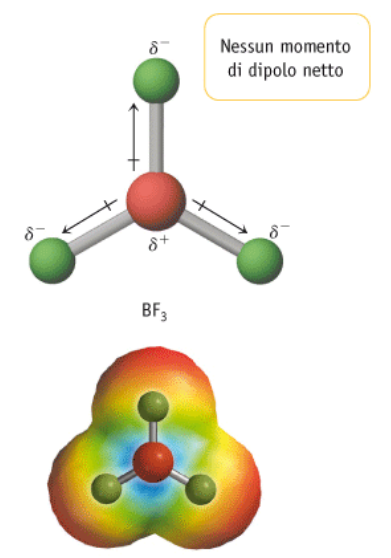
\includegraphics[width=5cm]{immagini/BF_3-dipolo.png}
\end{figure}

Nel descrivere tale molecola abbiamo detto che il boro presenta ibridizzazione sp$^2$, per cui essa sarà una molecola planare con angoli di 120°.

Il fluoro è parecchio più elettronegativo del boro, quindi ciascun legame mostrerà polarità, con la carica di legame addensata sul fluoro.

Essendo planare, la composizione dei tre momenti di dipolo, fra loro uguali in modulo, dà un momento di dipolo netto pari a zero, per cui il \ce{BF_3} non ha polarità. 

$\bullet$ ES8 \ce{Cl_2CO}

\begin{figure}[htp]
    \centering
    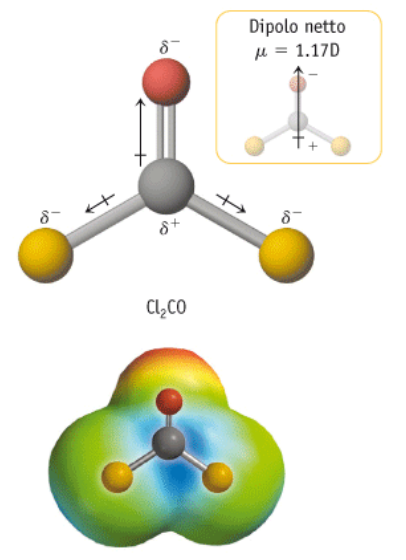
\includegraphics[width=5cm]{immagini/Cl_2CO.png}
\end{figure}
Nel fosgene un atomo di carbonio centrale è legato all'ossigeno tramite un doppio legame e a due atomi di cloro tramite due legami semplici. Sia il cloro che l'ossigeno sono parecchio più elettronegativi del carbonio, quindi ciascun legame mostrerà polarità con la freccia rivolta verso gli atomi esterni. Il momento di dipolo del legame carbonio-ossigeno è più forte, per cui la composizione darà un momento di dipolo netto pari a 1.17D.

$\bullet$ ES9 \ce{NH_3}

\begin{figure}[htp]
    \centering
    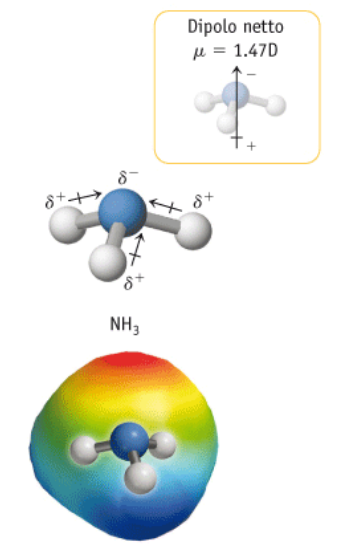
\includegraphics[width=5cm]{immagini/NH_3.png}
\end{figure}
Nell'ammoniaca è l'azoto centrale ad essere più elettronegativo, e lo è parecchio rispetto all'idrogeno. Ne segue che ogni legame mosterà polarità la cui freccia è rivolta verso questo. Inoltre col formalismo di Lewis abbiamo visto che su di esso è presente una coppia solitaria, la quale lo solleva dal piano dei tre atomi di idrogeno, per cui il momento di dipolo netto diverso da zero

$\bullet$ ES10

\begin{figure}[htp]
    \centering
    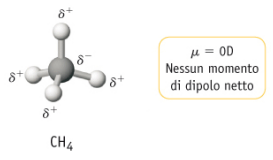
\includegraphics[width=5cm]{immagini/CH_4.png}
\end{figure}

$\bullet$ ES11

\begin{figure}[htp]
    \centering
    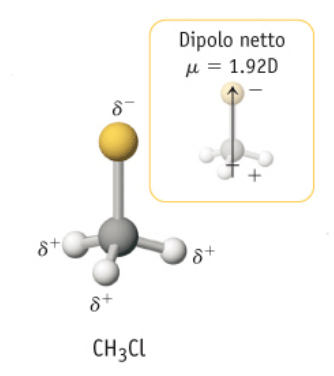
\includegraphics[width=5cm]{immagini/CH_3Cl.png}
\end{figure}

$\bullet$ ES12

\begin{figure}[htp]
    \centering
    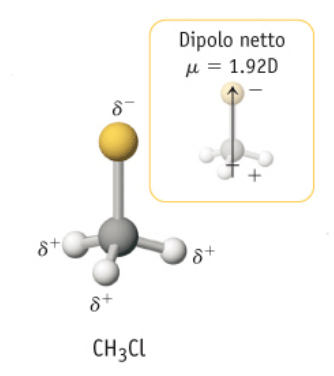
\includegraphics[width=5cm]{immagini/CH_3Cl.png}
\end{figure}

$\bullet$ ES13

\begin{figure}[htp]
    \centering
    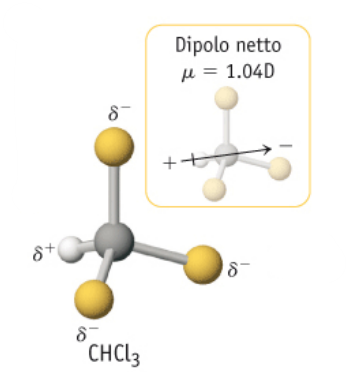
\includegraphics[width=5cm]{immagini/CHCl_3.png}
\end{figure}

$\bullet$ ES14

\begin{figure}[htp]
    \centering
    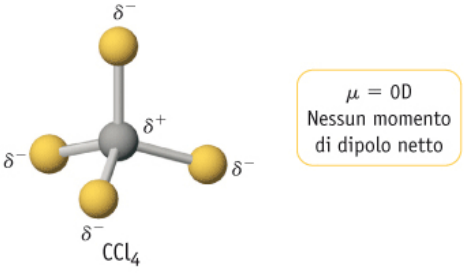
\includegraphics[width=5cm]{immagini/CCl_4.png}
\end{figure}
\subsection{Il legame ionico}
in esso la dislocazione delle cariche e totale, per cui immaginiamo che ci sia cessione dell'elettrone e in conseguenza a ciò si formino uno ione positivo e uno negativo.

\subsection{il ciclo di Born-Haber}

\subsection{Differenze tra composti molecolari e composti ionici}
Per i composti molecolari esistono le singole molecole, per quelli ionici no: essi esistono solo in forma di reticolo cristallino, dove gli ioni occupano posizioni ben precise, alternandosi, in tutte e 3 le direzioni.

La conseguenza di ciò è che se mettiamo in acqua ad esempio il glucosio \ce{C_6H_{12}O_6}, che è un composto molecolare, esso resta tale, mentre se mettiamo ad esempio il cloruro di sodio NaCl esso si dissocia in ioni Na$^+$ e Cl$^-$. Ciò che avviene è che l'acqua aggredisce il cristallo e stacca singoli ioni, i quali vengono portati in soluzione con delle molecole di acqua che li circondano. In particolare gli ioni positivi saranno circondati dagli atomi di ossigeno dell'acqua, in quanto essi reagiranno con la parziale carica negativa presente su questo, mentre gli ioni negativi saranno, mentre gli ioni negativi saranno circondati dagli idrogeni dell'acqua poiché interagiranno con la parziale carica positiva presente su questi:
\begin{figure}[htp]
    \centering
    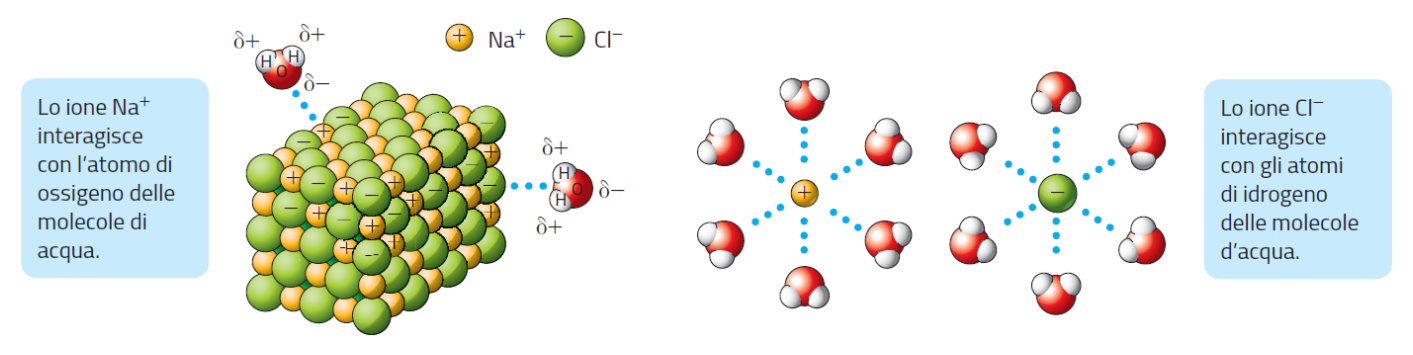
\includegraphics[width=15cm]{immagini/interazione-acqua-ioni.png}
\end{figure}
Dunque in soluzione si avranno ioni.

L'evidenza sperimentale di tale fatto si ottiene confrontando tre circuiti elettrici con una lampadina, dove in uno inseriamo in serie dell'NaCl solido, in un altro dell'NaCl fuso e in un terzo una soluzione di NaCl sciolto in acqua. Il primo non permette la conduzione (la lampada non si accende), il secondo permette una leggera conduzione (la lampada si accende ma la luce è fioca), il terzo permette una grande conduzione (la lampada si accende con luminosità maggiore).

\begin{figure}[htp]
    \centering
    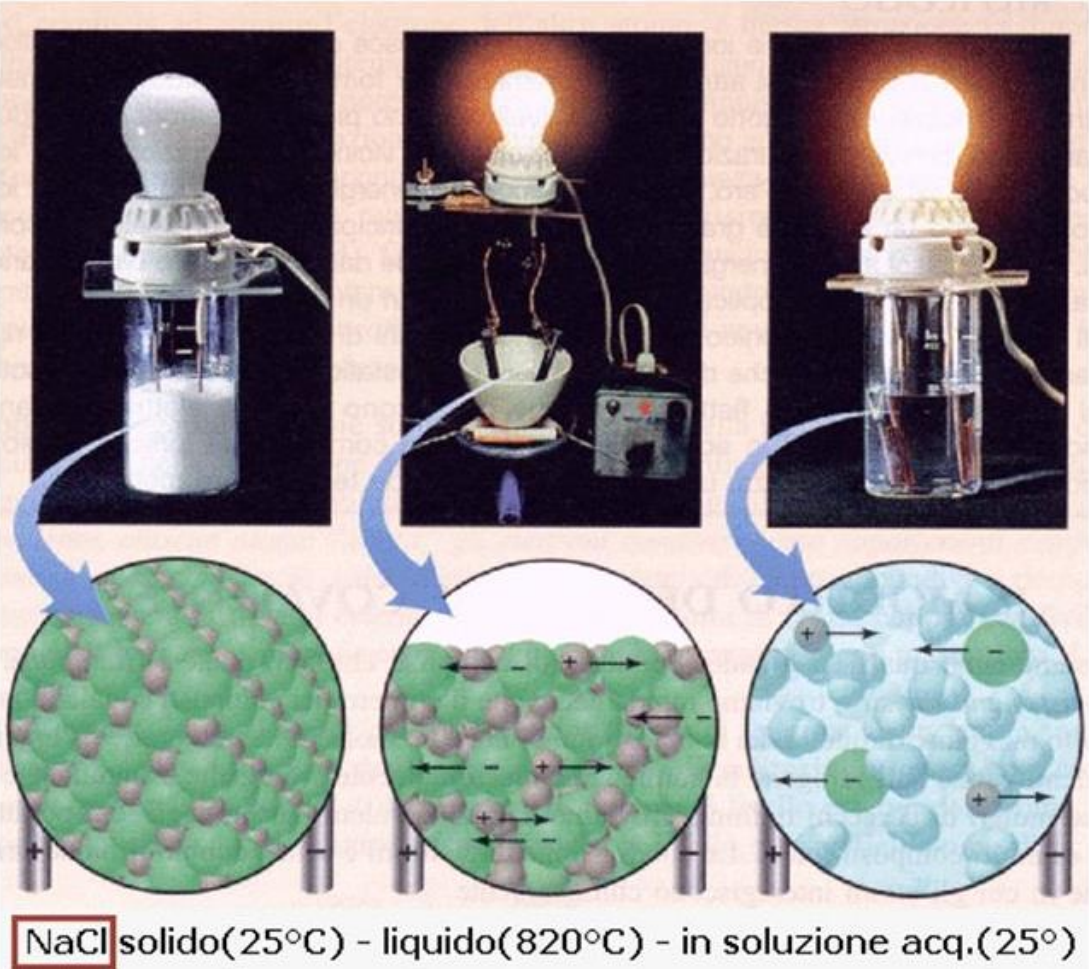
\includegraphics[width=10cm]{immagini/lampadina.png}
\end{figure}

Tale esperimento mostra l'esistenza degli ioni, che sono i portatori di carica che permettono la conduzione.

Se invece avessimo collegato a lampadina ad una soluzione acquosa contenente zucchero, la lampadina non si accenderebbe. Il motivo è che lo zucchero è un composto molecolare, per cui non si scioglie in acqua e non dà origine a ioni.
\subsection{Il legame covalente}
